
\captionsetup[subfigure]{labelformat=empty}

\begin{figure}[H] 
\centering
\caption{Components of the fitted modified Cholesky decomposition for the cattle weight data.}
\subfloat[Estimated Cholesky factor $\hat{T}$]{
  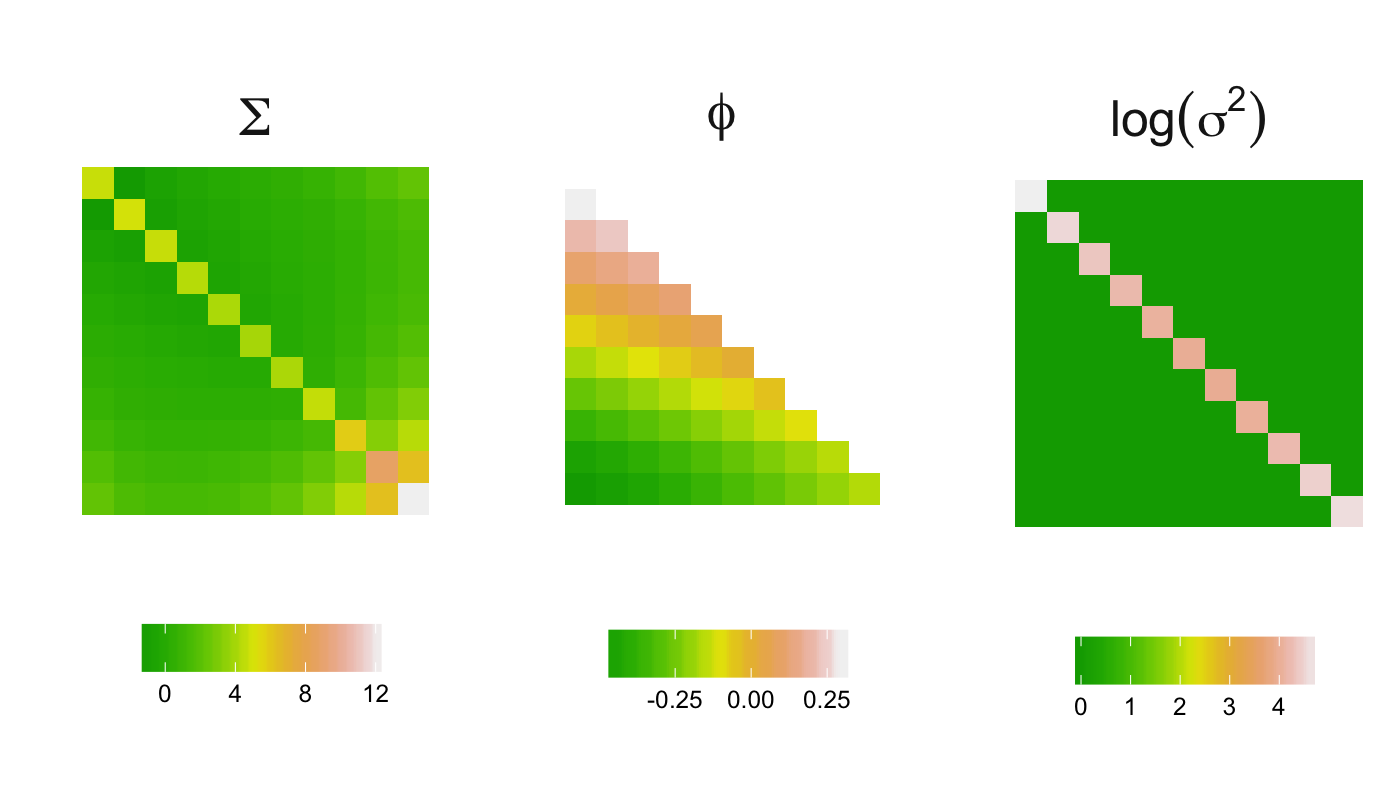
\includegraphics[width = .4\textwidth]{../img/chapter-5/cattle-cholesky-estimate-ggplot}
} \hfill
\subfloat[Estimated innovation variances \newline $\hat{D} = diag\left( \sigma^2\left(t_1\right),\dots, \sigma^2\left(t_{11}\right) \right)$]{
  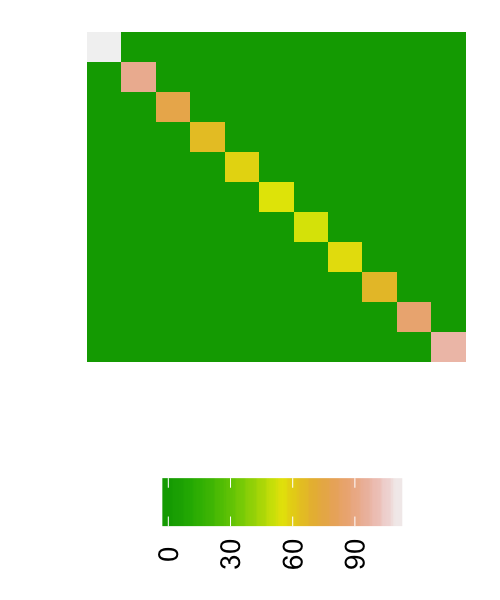
\includegraphics[width = .4\textwidth]{../img/chapter-5/cattle-D-estimate-ggplot}
} 
\hfill
\subfloat[Estimated covariance matrix $\hat{\Sigma} = \hat{T}^{-1} \hat{D} {\hat{T}'}^{-1}$]{
  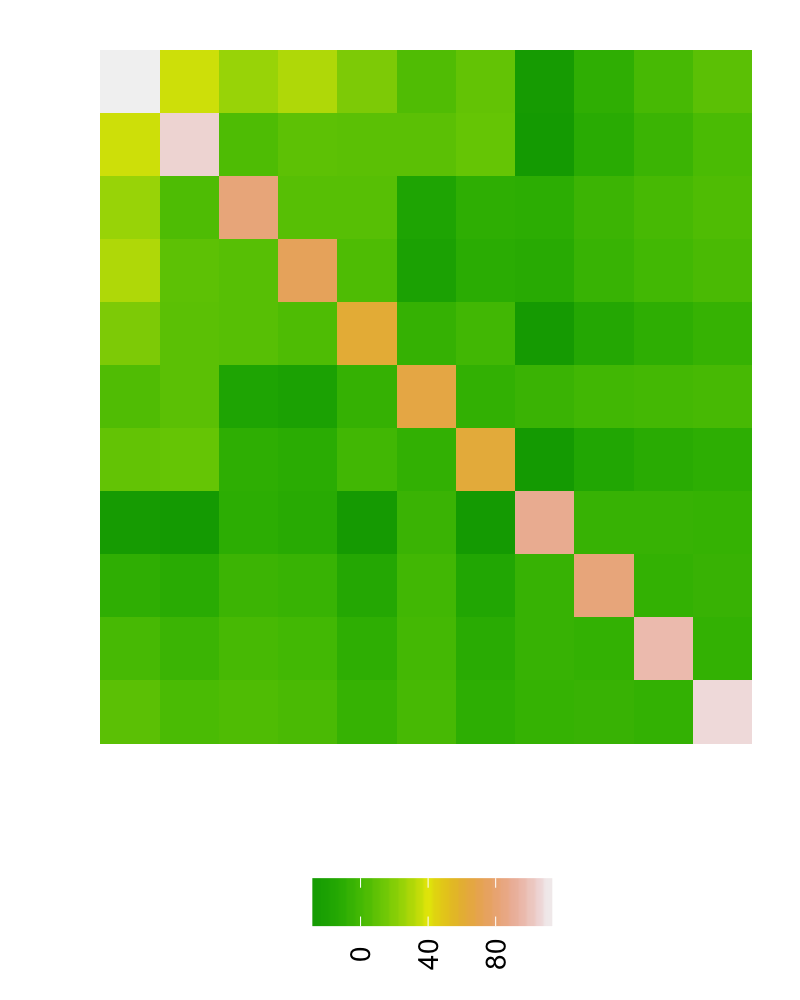
\includegraphics[width = .4\textwidth]{../img/chapter-5/cattle-cov-estimate-ggplot}
} 
\label{fig:cattle-fitted-cholesky-decomposition}
\end{figure}
